%%%%%%%%%%%%%%%%%%%%%%%%%%%%%%%%%%%%%%%%%%%%%%%%%%%%%%%%%%%%
% 3.11 CONVEX GEOMETRY
% The Composition of Advanced Mathematics
%%%%%%%%%%%%%%%%%%%%%%%%%%%%%%%%%%%%%%%%%%%%%%%%%%%%%%%%%%%%

\section{Convex Geometry}
\label{sec:convex-geometry}

\prerequisite{
Euclidean Geometry, Analytic Geometry, Vector Geometry,
Affine Geometry, and basic Linear Algebra.
}

\learningobjectives{
By the end of this section, the reader should be able to:
\begin{itemize}
    \item define convex sets and recognize common examples;
    \item test whether a set is convex;
    \item distinguish convex combinations from affine combinations;
    \item construct and interpret convex hulls;
    \item define extreme points and supporting hyperplanes;
    \item work with half-spaces and hyperplanes;
    \item define convex cones and polyhedral sets;
    \item distinguish polytopes and polyhedra;
    \item describe polytopes using vertices and inequalities;
    \item state and apply Carath\'eodory's theorem;
    \item explain Helly's theorem and Radon's theorem;
    \item state the hyperplane separation principle;
    \item define convex functions geometrically;
    \item explain the epigraph of a convex function;
    \item recognize strictly and strongly convex behavior;
    \item understand the geometric role of supporting functions;
    \item explain dual and polar convex sets;
    \item work with Minkowski sums;
    \item recognize basic volume and symmetry ideas in convex bodies;
    \item explain connections with optimization, computational geometry,
    probability, and functional analysis.
\end{itemize}
}

%%%%%%%%%%%%%%%%%%%%%%%%%%%%%%%%%%%%%%%%%%%%%%%%%%%%%%%%%%%%
\subsection{What Is Convex Geometry?}
\label{subsec:what-is-convex-geometry}
%%%%%%%%%%%%%%%%%%%%%%%%%%%%%%%%%%%%%%%%%%%%%%%%%%%%%%%%%%%%

Convex geometry studies geometric sets that contain the entire line segment
between any two of their points.

This apparently simple condition produces a remarkably rich theory.

Convexity appears throughout

\[
\boxed{
\text{geometry},
\quad
\text{optimization},
\quad
\text{linear algebra},
\quad
\text{analysis},
\quad
\text{probability},
\quad
\text{economics},
\quad
\text{data science}.
}
\]

The fundamental idea can be stated informally:

\begin{conceptbox}
A set is convex if traveling along a straight line from one point of the set
to another never requires leaving the set.
\end{conceptbox}

%%%%%%%%%%%%%%%%%%%%%%%%%%%%%%%%%%%%%%%%%%%%%%%%%%%%%%%%%%%%
\subsection{Line Segments in Vector Spaces}
\label{subsec:convex-line-segments}
%%%%%%%%%%%%%%%%%%%%%%%%%%%%%%%%%%%%%%%%%%%%%%%%%%%%%%%%%%%%

Let

\[
x,y\in\R^n.
\]

The line segment joining \(x\) and \(y\) consists of points

\[
\boxed{
(1-t)x+ty,
\qquad
0\leq t\leq1.
}
\]

When

\[
t=0,
\]

the point is \(x\), and when

\[
t=1,
\]

the point is \(y\).

Values between \(0\) and \(1\) trace the segment connecting them.

%%%%%%%%%%%%%%%%%%%%%%%%%%%%%%%%%%%%%%%%%%%%%%%%%%%%%%%%%%%%
\subsection{Convex Sets}
\label{subsec:convex-sets}
%%%%%%%%%%%%%%%%%%%%%%%%%%%%%%%%%%%%%%%%%%%%%%%%%%%%%%%%%%%%

\begin{definitionbox}{Convex Set}
A set

\[
C\subseteq\R^n
\]

is \emph{convex} if for every \(x,y\in C\) and every \(t\in[0,1]\),

\[
\boxed{
(1-t)x+ty\in C.
}
\]
\end{definitionbox}

Thus the complete segment between any two points of \(C\) lies inside \(C\).

%%%%%%%%%%%%%%%%%%%%%%%%%%%%%%%%%%%%%%%%%%%%%%%%%%%%%%%%%%%%
\subsection{Visualizing Convexity}
\label{subsec:visualizing-convexity}
%%%%%%%%%%%%%%%%%%%%%%%%%%%%%%%%%%%%%%%%%%%%%%%%%%%%%%%%%%%%

\begin{centereddiagram}
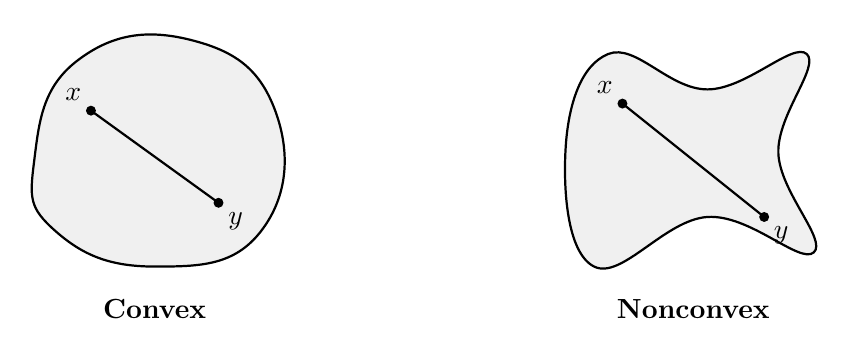
\begin{tikzpicture}[scale=.9]

% Convex
\begin{scope}[xshift=-3.8cm]
\draw[thick,fill=gray!12]
plot[smooth cycle,tension=.8]
coordinates{
(-1.7,0)
(-1.1,1.4)
(.5,1.7)
(1.7,.7)
(1.5,-1)
(0,-1.5)
(-1.4,-1)
};

\fill (-.9,.7) circle (2pt) node[above left] {$x$};
\fill (.9,-.6) circle (2pt) node[below right] {$y$};
\draw[thick] (-.9,.7)--(.9,-.6);

\node at (0,-2.1) {\textbf{Convex}};
\end{scope}

% Nonconvex
\begin{scope}[xshift=3.8cm]
\draw[thick,fill=gray!12]
plot[smooth cycle,tension=.7]
coordinates{
(-1.8,.2)
(-1.2,1.5)
(.2,1)
(1.6,1.5)
(1.2,.1)
(1.7,-1.3)
(.2,-.8)
(-1.4,-1.5)
};

\fill (-1,.8) circle (2pt) node[above left] {$x$};
\fill (1,-.8) circle (2pt) node[below right] {$y$};
\draw[thick] (-1,.8)--(1,-.8);

\node at (0,-2.1) {\textbf{Nonconvex}};
\end{scope}

\end{tikzpicture}
\end{centereddiagram}

For the convex set, every segment connecting points of the set remains
inside.

For the nonconvex set, some connecting segment leaves the set.

%%%%%%%%%%%%%%%%%%%%%%%%%%%%%%%%%%%%%%%%%%%%%%%%%%%%%%%%%%%%
\subsection{Basic Examples of Convex Sets}
\label{subsec:convex-basic-examples}
%%%%%%%%%%%%%%%%%%%%%%%%%%%%%%%%%%%%%%%%%%%%%%%%%%%%%%%%%%%%

Common convex sets include:

\[
\boxed{\R^n}
\]

and the empty set,

\[
\boxed{\varnothing}.
\]

Every affine subspace is convex.

Every line and line segment is convex.

Every closed Euclidean ball

\[
\boxed{
B=
\{x\in\R^n:\|x-c\|\leq r\}
}
\]

is convex.

Every half-space is convex.

Triangles, rectangles, and ordinary solid polygons without inward
indentations are convex.

%%%%%%%%%%%%%%%%%%%%%%%%%%%%%%%%%%%%%%%%%%%%%%%%%%%%%%%%%%%%
\subsection{Examples of Nonconvex Sets}
\label{subsec:nonconvex-examples}
%%%%%%%%%%%%%%%%%%%%%%%%%%%%%%%%%%%%%%%%%%%%%%%%%%%%%%%%%%%%

A circle considered only as its boundary,

\[
\boxed{
\{x\in\R^2:\|x\|=1\},
}
\]

is not convex.

Two disconnected disks are generally not convex.

An annulus

\[
\boxed{
\{x\in\R^2:1\leq\|x\|\leq2\}
}
\]

is not convex because a segment between opposite points may pass through the
missing center.

A polygon containing an inward indentation is not convex.

%%%%%%%%%%%%%%%%%%%%%%%%%%%%%%%%%%%%%%%%%%%%%%%%%%%%%%%%%%%%
\subsection{Testing Convexity}
\label{subsec:testing-convexity}
%%%%%%%%%%%%%%%%%%%%%%%%%%%%%%%%%%%%%%%%%%%%%%%%%%%%%%%%%%%%

To prove that \(C\) is convex, begin with arbitrary

\[
x,y\in C
\]

and

\[
t\in[0,1].
\]

Then show that

\[
\boxed{
(1-t)x+ty\in C.
}
\]

To prove that a set is not convex, it is enough to find

\[
x,y\in C
\]

and some

\[
t\in(0,1)
\]

such that

\[
\boxed{
(1-t)x+ty\notin C.
}
\]

%%%%%%%%%%%%%%%%%%%%%%%%%%%%%%%%%%%%%%%%%%%%%%%%%%%%%%%%%%%%
\subsection{Worked Example: A Convex Interval}
\label{subsec:worked-convex-interval}
%%%%%%%%%%%%%%%%%%%%%%%%%%%%%%%%%%%%%%%%%%%%%%%%%%%%%%%%%%%%

\begin{workedexamplebox}{Prove That an Interval Is Convex}

Consider

\[
C=[a,b]\subseteq\R.
\]

Take

\[
x,y\in[a,b]
\]

and

\[
t\in[0,1].
\]

Since

\[
a\leq x\leq b
\]

and

\[
a\leq y\leq b,
\]

multiplying by the nonnegative quantities \(1-t\) and \(t\) gives

\[
(1-t)a\leq(1-t)x\leq(1-t)b
\]

and

\[
ta\leq ty\leq tb.
\]

Adding,

\[
a
\leq
(1-t)x+ty
\leq
b.
\]

Therefore

\[
(1-t)x+ty\in[a,b].
\]

\begin{answerbox}
\[
\boxed{
[a,b]\text{ is convex.}
}
\]
\end{answerbox}
\end{workedexamplebox}

%%%%%%%%%%%%%%%%%%%%%%%%%%%%%%%%%%%%%%%%%%%%%%%%%%%%%%%%%%%%
\subsection{Worked Example: A Nonconvex Set}
\label{subsec:worked-nonconvex-set}
%%%%%%%%%%%%%%%%%%%%%%%%%%%%%%%%%%%%%%%%%%%%%%%%%%%%%%%%%%%%

\begin{workedexamplebox}{Show That the Unit Circle Is Not Convex}

Consider

\[
C=
\{(x,y)\in\R^2:x^2+y^2=1\}.
\]

Choose

\[
u=(1,0)
\]

and

\[
v=(-1,0).
\]

Both belong to \(C\).

Their midpoint is

\[
\frac12u+\frac12v
=
(0,0).
\]

But

\[
0^2+0^2\neq1.
\]

Thus

\[
(0,0)\notin C.
\]

\begin{answerbox}
\[
\boxed{
C\text{ is not convex.}
}
\]
\end{answerbox}
\end{workedexamplebox}

%%%%%%%%%%%%%%%%%%%%%%%%%%%%%%%%%%%%%%%%%%%%%%%%%%%%%%%%%%%%
\subsection{Convex Combinations}
\label{subsec:convex-combinations}
%%%%%%%%%%%%%%%%%%%%%%%%%%%%%%%%%%%%%%%%%%%%%%%%%%%%%%%%%%%%

\begin{definitionbox}{Convex Combination}
A \emph{convex combination} of points

\[
x_1,\ldots,x_m
\]

is an expression

\[
\boxed{
\lambda_1x_1+\cdots+\lambda_mx_m
}
\]

where

\[
\boxed{
\lambda_i\geq0
}
\]

and

\[
\boxed{
\lambda_1+\cdots+\lambda_m=1.
}
\]
\end{definitionbox}

The lowercase Greek letter

\[
\lambda
\]

is read ``lambda.''

The coefficients \(\lambda_i\) are called \emph{weights}.

%%%%%%%%%%%%%%%%%%%%%%%%%%%%%%%%%%%%%%%%%%%%%%%%%%%%%%%%%%%%
\subsection{Convex Versus Affine Combinations}
\label{subsec:convex-vs-affine-combinations}
%%%%%%%%%%%%%%%%%%%%%%%%%%%%%%%%%%%%%%%%%%%%%%%%%%%%%%%%%%%%

An affine combination satisfies

\[
\sum_{i=1}^{m}\lambda_i=1,
\]

but the coefficients may be negative.

A convex combination additionally requires

\[
\boxed{
\lambda_i\geq0.
}
\]

Therefore,

\[
\boxed{
\text{convex combination}
\Longrightarrow
\text{affine combination}.
}
\]

The converse is not generally true.

%%%%%%%%%%%%%%%%%%%%%%%%%%%%%%%%%%%%%%%%%%%%%%%%%%%%%%%%%%%%
\subsection{Characterization by Convex Combinations}
\label{subsec:convex-combination-characterization}
%%%%%%%%%%%%%%%%%%%%%%%%%%%%%%%%%%%%%%%%%%%%%%%%%%%%%%%%%%%%

A set \(C\) is convex if and only if every finite convex combination of
points of \(C\) remains in \(C\).

Thus if

\[
x_1,\ldots,x_m\in C,
\]

then

\[
\boxed{
\sum_{i=1}^{m}\lambda_ix_i\in C
}
\]

whenever

\[
\lambda_i\geq0
\]

and

\[
\sum_i\lambda_i=1.
\]

%%%%%%%%%%%%%%%%%%%%%%%%%%%%%%%%%%%%%%%%%%%%%%%%%%%%%%%%%%%%
\subsection{Convex Hulls}
\label{subsec:convex-hulls}
%%%%%%%%%%%%%%%%%%%%%%%%%%%%%%%%%%%%%%%%%%%%%%%%%%%%%%%%%%%%

\begin{definitionbox}{Convex Hull}
The \emph{convex hull} of a set \(S\subseteq\R^n\), written

\[
\boxed{
\operatorname{conv}(S),
}
\]

is the smallest convex set containing \(S\).
\end{definitionbox}

Equivalently,

\[
\boxed{
\operatorname{conv}(S)
=
\left\{
\sum_{i=1}^{m}\lambda_ix_i:
x_i\in S,\;
\lambda_i\geq0,\;
\sum_{i=1}^{m}\lambda_i=1
\right\}.
}
\]

%%%%%%%%%%%%%%%%%%%%%%%%%%%%%%%%%%%%%%%%%%%%%%%%%%%%%%%%%%%%
\subsection{Geometric Meaning of the Convex Hull}
\label{subsec:convex-hull-geometric-meaning}
%%%%%%%%%%%%%%%%%%%%%%%%%%%%%%%%%%%%%%%%%%%%%%%%%%%%%%%%%%%%

Informally, imagine placing an elastic band around a collection of points.

When released, the band contracts around the outermost points.

The enclosed region represents their convex hull.

\begin{centereddiagram}
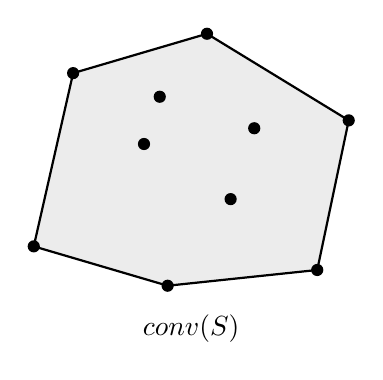
\begin{tikzpicture}[scale=1]

\coordinate (A) at (-2,-1);
\coordinate (B) at (-1.5,1.2);
\coordinate (C) at (.2,1.7);
\coordinate (D) at (2,.6);
\coordinate (E) at (1.6,-1.3);
\coordinate (F) at (-.3,-1.5);

\fill[gray!15]
(A)--(B)--(C)--(D)--(E)--(F)--cycle;

\draw[thick]
(A)--(B)--(C)--(D)--(E)--(F)--cycle;

\foreach \P in {A,B,C,D,E,F}
    \fill (\P) circle (2.2pt);

\fill (-.6,.3) circle (2.2pt);
\fill (.5,-.4) circle (2.2pt);
\fill (.8,.5) circle (2.2pt);
\fill (-.4,.9) circle (2.2pt);

\node at (0,-2.05) {$\operatorname{conv}(S)$};

\end{tikzpicture}
\end{centereddiagram}

Interior points do not affect the outer boundary of the convex hull.

%%%%%%%%%%%%%%%%%%%%%%%%%%%%%%%%%%%%%%%%%%%%%%%%%%%%%%%%%%%%
\subsection{Intersection of Convex Sets}
\label{subsec:intersection-convex-sets}
%%%%%%%%%%%%%%%%%%%%%%%%%%%%%%%%%%%%%%%%%%%%%%%%%%%%%%%%%%%%

\begin{theorem}
The intersection of any collection of convex sets is convex.
\end{theorem}

Suppose

\[
C=\bigcap_{\alpha}C_\alpha
\]

where every \(C_\alpha\) is convex.

If

\[
x,y\in C,
\]

then \(x,y\) belong to every \(C_\alpha\).

Therefore

\[
(1-t)x+ty\in C_\alpha
\]

for every \(\alpha\).

Hence

\[
\boxed{
(1-t)x+ty\in C.
}
\]

%%%%%%%%%%%%%%%%%%%%%%%%%%%%%%%%%%%%%%%%%%%%%%%%%%%%%%%%%%%%
\subsection{Unions Need Not Be Convex}
\label{subsec:union-convex-sets}
%%%%%%%%%%%%%%%%%%%%%%%%%%%%%%%%%%%%%%%%%%%%%%%%%%%%%%%%%%%%

The union of convex sets need not be convex.

For example, two disjoint disks are individually convex, but their union is
not convex.

Thus

\[
\boxed{
C_1,C_2\text{ convex}
\not\Longrightarrow
C_1\cup C_2\text{ convex}.
}
\]

%%%%%%%%%%%%%%%%%%%%%%%%%%%%%%%%%%%%%%%%%%%%%%%%%%%%%%%%%%%%
\subsection{Affine Images of Convex Sets}
\label{subsec:affine-images-convex}
%%%%%%%%%%%%%%%%%%%%%%%%%%%%%%%%%%%%%%%%%%%%%%%%%%%%%%%%%%%%

Let

\[
T(x)=Ax+b
\]

be an affine transformation.

If \(C\) is convex, then

\[
\boxed{
T(C)
}
\]

is convex.

Indeed,

\[
T((1-t)x+ty)
=
(1-t)T(x)+tT(y).
\]

Therefore affine transformations preserve convexity.

This explains the close relationship between convex geometry and affine
geometry.

%%%%%%%%%%%%%%%%%%%%%%%%%%%%%%%%%%%%%%%%%%%%%%%%%%%%%%%%%%%%
\subsection{Hyperplanes}
\label{subsec:convex-hyperplanes}
%%%%%%%%%%%%%%%%%%%%%%%%%%%%%%%%%%%%%%%%%%%%%%%%%%%%%%%%%%%%

A hyperplane in \(\R^n\) has the form

\[
\boxed{
H=
\{x\in\R^n:a\cdot x=b\},
}
\]

where

\[
a\neq0.
\]

The vector \(a\) is normal to the hyperplane.

In \(\R^2\), a hyperplane is a line.

In \(\R^3\), a hyperplane is a plane.

%%%%%%%%%%%%%%%%%%%%%%%%%%%%%%%%%%%%%%%%%%%%%%%%%%%%%%%%%%%%
\subsection{Half-Spaces}
\label{subsec:convex-halfspaces}
%%%%%%%%%%%%%%%%%%%%%%%%%%%%%%%%%%%%%%%%%%%%%%%%%%%%%%%%%%%%

A hyperplane divides space into two half-spaces.

The closed half-spaces are

\[
\boxed{
H^-=
\{x:a\cdot x\leq b\}
}
\]

and

\[
\boxed{
H^+=
\{x:a\cdot x\geq b\}.
}
\]

Both are convex.

%%%%%%%%%%%%%%%%%%%%%%%%%%%%%%%%%%%%%%%%%%%%%%%%%%%%%%%%%%%%
\subsection{Supporting Hyperplanes}
\label{subsec:supporting-hyperplanes}
%%%%%%%%%%%%%%%%%%%%%%%%%%%%%%%%%%%%%%%%%%%%%%%%%%%%%%%%%%%%

\begin{definitionbox}{Supporting Hyperplane}
Let \(C\subseteq\R^n\) be convex.

A hyperplane

\[
H=\{x:a\cdot x=b\}
\]

is a \emph{supporting hyperplane} of \(C\) if

\[
C
\]

lies entirely in one of the corresponding closed half-spaces and

\[
\boxed{
C\cap H\neq\varnothing.
}
\]
\end{definitionbox}

A supporting hyperplane touches a convex set without cutting through its
interior.

\begin{centereddiagram}
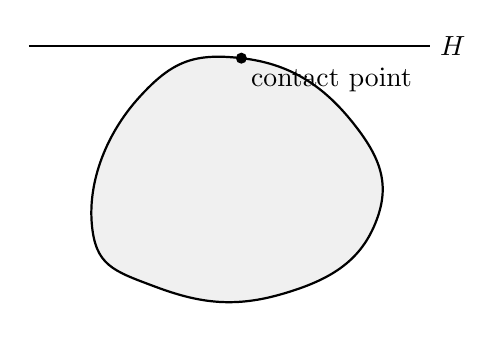
\begin{tikzpicture}[scale=1]

\draw[thick,fill=gray!12]
plot[smooth cycle,tension=.8]
coordinates{
(-1.8,-.5)
(-1.2,1.1)
(.1,1.6)
(1.5,.8)
(1.8,-.5)
(.6,-1.4)
(-1,-1.3)
};

\draw[thick] (-2.6,1.75)--(2.5,1.75);
\node[right] at (2.5,1.75) {$H$};

\fill (.1,1.6) circle (2pt);
\node[below right] at (.1,1.6) {contact point};

\end{tikzpicture}
\end{centereddiagram}

%%%%%%%%%%%%%%%%%%%%%%%%%%%%%%%%%%%%%%%%%%%%%%%%%%%%%%%%%%%%
\subsection{Extreme Points}
\label{subsec:extreme-points}
%%%%%%%%%%%%%%%%%%%%%%%%%%%%%%%%%%%%%%%%%%%%%%%%%%%%%%%%%%%%

\begin{definitionbox}{Extreme Point}
A point \(x\in C\) is an \emph{extreme point} of a convex set \(C\) if it
cannot be written as

\[
\boxed{
x=(1-t)y+tz
}
\]

for distinct \(y,z\in C\) and \(0<t<1\).
\end{definitionbox}

Intuitively, extreme points are the ``corners'' or irreducible boundary
points of a convex set.

For a triangle, the three vertices are its extreme points.

For a closed disk, every point on the boundary circle is an extreme point.

%%%%%%%%%%%%%%%%%%%%%%%%%%%%%%%%%%%%%%%%%%%%%%%%%%%%%%%%%%%%
\subsection{Faces}
\label{subsec:convex-faces}
%%%%%%%%%%%%%%%%%%%%%%%%%%%%%%%%%%%%%%%%%%%%%%%%%%%%%%%%%%%%

A supporting hyperplane determines part of the boundary of a convex set.

\begin{definitionbox}{Face}
A \emph{face} of a convex set \(C\) is a subset obtained by intersecting
\(C\) with a supporting hyperplane:

\[
\boxed{
F=C\cap H.
}
\]
\end{definitionbox}

For a three-dimensional polytope, familiar examples include:

\[
\boxed{
\text{vertices},
\quad
\text{edges},
\quad
\text{two-dimensional faces}.
}
\]

%%%%%%%%%%%%%%%%%%%%%%%%%%%%%%%%%%%%%%%%%%%%%%%%%%%%%%%%%%%%
\subsection{Convex Cones}
\label{subsec:convex-cones}
%%%%%%%%%%%%%%%%%%%%%%%%%%%%%%%%%%%%%%%%%%%%%%%%%%%%%%%%%%%%

\begin{definitionbox}{Convex Cone}
A set \(K\subseteq\R^n\) is a \emph{convex cone} if

\[
x,y\in K,
\qquad
\alpha,\beta\geq0
\]

imply

\[
\boxed{
\alpha x+\beta y\in K.
}
\]
\end{definitionbox}

In particular, if \(x\in K\), then

\[
\boxed{
\lambda x\in K
\qquad
\text{for every }\lambda\geq0.
}
\]

%%%%%%%%%%%%%%%%%%%%%%%%%%%%%%%%%%%%%%%%%%%%%%%%%%%%%%%%%%%%
\subsection{Conic Hulls}
\label{subsec:conic-hulls}
%%%%%%%%%%%%%%%%%%%%%%%%%%%%%%%%%%%%%%%%%%%%%%%%%%%%%%%%%%%%

The \emph{conic hull} of vectors

\[
v_1,\ldots,v_m
\]

is

\[
\boxed{
\operatorname{cone}(v_1,\ldots,v_m)
=
\left\{
\sum_{i=1}^{m}\lambda_iv_i:
\lambda_i\geq0
\right\}.
}
\]

Unlike a convex combination, the coefficients do not need to sum to \(1\).

%%%%%%%%%%%%%%%%%%%%%%%%%%%%%%%%%%%%%%%%%%%%%%%%%%%%%%%%%%%%
\subsection{Polyhedra}
\label{subsec:polyhedra}
%%%%%%%%%%%%%%%%%%%%%%%%%%%%%%%%%%%%%%%%%%%%%%%%%%%%%%%%%%%%

\begin{definitionbox}{Polyhedron}
A \emph{polyhedron} is an intersection of finitely many closed half-spaces.
\end{definitionbox}

Thus a polyhedron can be written as

\[
\boxed{
P=
\{x\in\R^n:Ax\leq b\}.
}
\]

Since half-spaces are convex and intersections of convex sets are convex,

\[
\boxed{
\text{every polyhedron is convex}.
}
\]

A polyhedron may be bounded or unbounded.

%%%%%%%%%%%%%%%%%%%%%%%%%%%%%%%%%%%%%%%%%%%%%%%%%%%%%%%%%%%%
\subsection{Polytopes}
\label{subsec:polytopes}
%%%%%%%%%%%%%%%%%%%%%%%%%%%%%%%%%%%%%%%%%%%%%%%%%%%%%%%%%%%%

\begin{definitionbox}{Polytope}
A \emph{polytope} is the convex hull of finitely many points:

\[
\boxed{
P=
\operatorname{conv}
\{v_1,\ldots,v_m\}.
}
\]
\end{definitionbox}

Every polytope is bounded.

Examples include:

\[
\boxed{
\text{line segments},
\quad
\text{triangles},
\quad
\text{polygons},
\quad
\text{tetrahedra},
\quad
\text{cubes}.
}
\]

%%%%%%%%%%%%%%%%%%%%%%%%%%%%%%%%%%%%%%%%%%%%%%%%%%%%%%%%%%%%
\subsection{Vertex and Half-Space Descriptions}
\label{subsec:vertex-halfspace-descriptions}
%%%%%%%%%%%%%%%%%%%%%%%%%%%%%%%%%%%%%%%%%%%%%%%%%%%%%%%%%%%%

A polytope may often be described in two complementary ways.

The \emph{vertex description}, or \(V\)-representation, is

\[
\boxed{
P=
\operatorname{conv}\{v_1,\ldots,v_m\}.
}
\]

The \emph{half-space description}, or \(H\)-representation, is

\[
\boxed{
P=
\{x:Ax\leq b\}.
}
\]

These two descriptions are fundamental in computational geometry and linear
optimization.

%%%%%%%%%%%%%%%%%%%%%%%%%%%%%%%%%%%%%%%%%%%%%%%%%%%%%%%%%%%%
\subsection{Minkowski--Weyl Theorem}
\label{subsec:minkowski-weyl}
%%%%%%%%%%%%%%%%%%%%%%%%%%%%%%%%%%%%%%%%%%%%%%%%%%%%%%%%%%%%

A central theorem connects finite geometric generation with systems of
linear inequalities.

\begin{theorem}[Minkowski--Weyl Theorem]
A set \(P\subseteq\R^n\) is a polyhedron if and only if it can be written as

\[
\boxed{
P=
\operatorname{conv}\{v_1,\ldots,v_k\}
+
\operatorname{cone}\{r_1,\ldots,r_m\}.
}
\]
\end{theorem}

The vectors \(r_i\) describe the unbounded directions of the polyhedron.

For a bounded polyhedron, no nonzero recession directions are needed, and
the set is a polytope.

%%%%%%%%%%%%%%%%%%%%%%%%%%%%%%%%%%%%%%%%%%%%%%%%%%%%%%%%%%%%
\subsection{Simplices}
\label{subsec:convex-simplices}
%%%%%%%%%%%%%%%%%%%%%%%%%%%%%%%%%%%%%%%%%%%%%%%%%%%%%%%%%%%%

A simplex is the higher-dimensional analogue of a triangle.

In dimension \(n\), an \(n\)-simplex is the convex hull of \(n+1\) affinely
independent points:

\[
\boxed{
\Delta
=
\operatorname{conv}
\{v_0,\ldots,v_n\}.
}
\]

Examples are:

\[
\begin{array}{c|c}
n & n\text{-simplex}\\
\hline
0 & \text{point}\\
1 & \text{line segment}\\
2 & \text{triangle}\\
3 & \text{tetrahedron}
\end{array}
\]

%%%%%%%%%%%%%%%%%%%%%%%%%%%%%%%%%%%%%%%%%%%%%%%%%%%%%%%%%%%%
\subsection{Barycentric Coordinates}
\label{subsec:convex-barycentric-coordinates}
%%%%%%%%%%%%%%%%%%%%%%%%%%%%%%%%%%%%%%%%%%%%%%%%%%%%%%%%%%%%

A point \(x\) in a simplex can be written as

\[
\boxed{
x=
\lambda_0v_0+\cdots+\lambda_nv_n
}
\]

where

\[
\lambda_i\geq0
\]

and

\[
\boxed{
\sum_{i=0}^{n}\lambda_i=1.
}
\]

The coefficients

\[
\lambda_0,\ldots,\lambda_n
\]

are the barycentric coordinates of \(x\) relative to the simplex.

%%%%%%%%%%%%%%%%%%%%%%%%%%%%%%%%%%%%%%%%%%%%%%%%%%%%%%%%%%%%
\subsection{Carath\'eodory's Theorem}
\label{subsec:caratheodory-theorem}
%%%%%%%%%%%%%%%%%%%%%%%%%%%%%%%%%%%%%%%%%%%%%%%%%%%%%%%%%%%%

Although a convex hull may be generated by many points, each individual
point requires only a limited number of them.

\begin{theorem}[Carath\'eodory's Theorem]
If

\[
x\in\operatorname{conv}(S)
\]

for some

\[
S\subseteq\R^n,
\]

then there exist at most \(n+1\) points

\[
x_0,\ldots,x_n\in S
\]

such that

\[
\boxed{
x\in
\operatorname{conv}\{x_0,\ldots,x_n\}.
}
\]
\end{theorem}

Thus every point in a planar convex hull requires at most three generating
points.

Every point in a convex hull in \(\R^3\) requires at most four.

%%%%%%%%%%%%%%%%%%%%%%%%%%%%%%%%%%%%%%%%%%%%%%%%%%%%%%%%%%%%
\subsection{Radon's Theorem}
\label{subsec:radon-theorem}
%%%%%%%%%%%%%%%%%%%%%%%%%%%%%%%%%%%%%%%%%%%%%%%%%%%%%%%%%%%%

\begin{theorem}[Radon's Theorem]
Any collection of \(n+2\) points in \(\R^n\) can be partitioned into two
disjoint subsets whose convex hulls intersect.
\end{theorem}

Symbolically, there exists a partition

\[
S=A\cup B,
\qquad
A\cap B=\varnothing,
\]

such that

\[
\boxed{
\operatorname{conv}(A)
\cap
\operatorname{conv}(B)
\neq
\varnothing.
}
\]

Radon's theorem is one of the foundational results of combinatorial convex
geometry.

%%%%%%%%%%%%%%%%%%%%%%%%%%%%%%%%%%%%%%%%%%%%%%%%%%%%%%%%%%%%
\subsection{Helly's Theorem}
\label{subsec:helly-theorem}
%%%%%%%%%%%%%%%%%%%%%%%%%%%%%%%%%%%%%%%%%%%%%%%%%%%%%%%%%%%%

Helly's theorem gives a powerful local-to-global intersection principle.

\begin{theorem}[Helly's Theorem]
Let

\[
C_1,\ldots,C_m
\]

be convex subsets of \(\R^n\), with

\[
m\geq n+1.
\]

If every \(n+1\) of these sets have nonempty intersection, then

\[
\boxed{
\bigcap_{i=1}^{m}C_i\neq\varnothing.
}
\]
\end{theorem}

In the plane, it is enough to check every collection of three convex sets.

%%%%%%%%%%%%%%%%%%%%%%%%%%%%%%%%%%%%%%%%%%%%%%%%%%%%%%%%%%%%
\subsection{Separation of Convex Sets}
\label{subsec:convex-separation}
%%%%%%%%%%%%%%%%%%%%%%%%%%%%%%%%%%%%%%%%%%%%%%%%%%%%%%%%%%%%

One of the most important principles in convex geometry is that disjoint
convex sets can often be separated by hyperplanes.

Geometrically, a hyperplane can be placed between the sets so that they lie
on opposite sides.

\begin{centereddiagram}
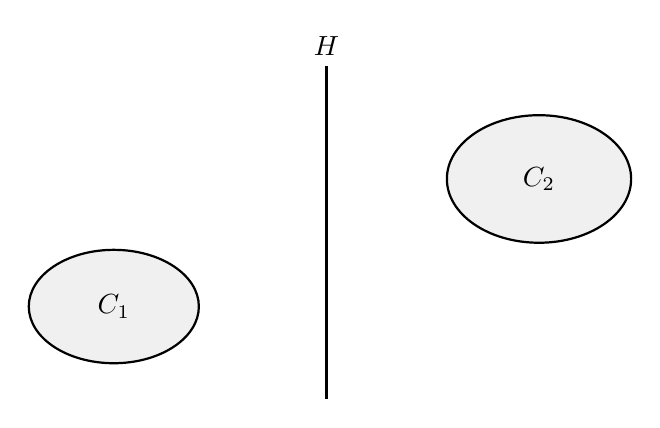
\begin{tikzpicture}[scale=.9]

\draw[thick,fill=gray!12]
(-3,-1) ellipse (1.2 and .8);

\draw[thick,fill=gray!12]
(3,.8) ellipse (1.3 and .9);

\draw[thick] (0,-2.3)--(0,2.4);
\node[above] at (0,2.4) {$H$};

\node at (-3,-1) {$C_1$};
\node at (3,.8) {$C_2$};

\end{tikzpicture}
\end{centereddiagram}

%%%%%%%%%%%%%%%%%%%%%%%%%%%%%%%%%%%%%%%%%%%%%%%%%%%%%%%%%%%%
\subsection{Strict Separation}
\label{subsec:strict-separation}
%%%%%%%%%%%%%%%%%%%%%%%%%%%%%%%%%%%%%%%%%%%%%%%%%%%%%%%%%%%%

Under suitable hypotheses, two disjoint convex sets can be strictly
separated.

This means there exist

\[
a\neq0
\]

and \(b\in\R\) such that

\[
\boxed{
a\cdot x<b<a\cdot y
}
\]

for all

\[
x\in C_1,
\qquad
y\in C_2.
\]

The exact hypotheses required depend on whether the sets are open, closed,
compact, or unbounded.

%%%%%%%%%%%%%%%%%%%%%%%%%%%%%%%%%%%%%%%%%%%%%%%%%%%%%%%%%%%%
\subsection{Point--Set Separation}
\label{subsec:point-set-separation}
%%%%%%%%%%%%%%%%%%%%%%%%%%%%%%%%%%%%%%%%%%%%%%%%%%%%%%%%%%%%

A particularly useful case occurs when

\[
x_0\notin C
\]

and \(C\) is a nonempty closed convex set.

Then there exists a hyperplane separating \(x_0\) from \(C\).

Under standard finite-dimensional hypotheses, one can find \(a\neq0\) and
\(b\) such that

\[
\boxed{
a\cdot x_0>b
}
\]

while

\[
\boxed{
a\cdot x\leq b
\qquad
\text{for all }x\in C.
}
\]

This principle is fundamental in convex optimization.

%%%%%%%%%%%%%%%%%%%%%%%%%%%%%%%%%%%%%%%%%%%%%%%%%%%%%%%%%%%%
\subsection{Nearest Points and Projection}
\label{subsec:convex-projection}
%%%%%%%%%%%%%%%%%%%%%%%%%%%%%%%%%%%%%%%%%%%%%%%%%%%%%%%%%%%%

Let \(C\subseteq\R^n\) be nonempty, closed, and convex.

For every \(x\in\R^n\), there exists a unique point

\[
P_C(x)\in C
\]

minimizing the Euclidean distance to \(x\):

\[
\boxed{
\|x-P_C(x)\|
=
\min_{y\in C}\|x-y\|.
}
\]

The point

\[
P_C(x)
\]

is called the \emph{metric projection} of \(x\) onto \(C\).

%%%%%%%%%%%%%%%%%%%%%%%%%%%%%%%%%%%%%%%%%%%%%%%%%%%%%%%%%%%%
\subsection{Projection Characterization}
\label{subsec:convex-projection-characterization}
%%%%%%%%%%%%%%%%%%%%%%%%%%%%%%%%%%%%%%%%%%%%%%%%%%%%%%%%%%%%

For a closed convex set \(C\),

\[
p=P_C(x)
\]

if and only if

\[
\boxed{
(x-p)\cdot(y-p)\leq0
\qquad
\text{for every }y\in C.
}
\]

Thus the displacement from the projection point toward \(x\) determines a
supporting direction for the convex set.

%%%%%%%%%%%%%%%%%%%%%%%%%%%%%%%%%%%%%%%%%%%%%%%%%%%%%%%%%%%%
\subsection{Convex Bodies}
\label{subsec:convex-bodies}
%%%%%%%%%%%%%%%%%%%%%%%%%%%%%%%%%%%%%%%%%%%%%%%%%%%%%%%%%%%%

\begin{definitionbox}{Convex Body}
A \emph{convex body} in \(\R^n\) is a compact convex set with nonempty
interior.
\end{definitionbox}

Examples include:

\[
\boxed{
\text{closed balls},
\quad
\text{solid ellipsoids},
\quad
\text{solid cubes},
\quad
\text{full-dimensional polytopes}.
}
\]

Convex bodies are central objects in classical convex geometry.

%%%%%%%%%%%%%%%%%%%%%%%%%%%%%%%%%%%%%%%%%%%%%%%%%%%%%%%%%%%%
\subsection{Strictly Convex Sets}
\label{subsec:strictly-convex-sets}
%%%%%%%%%%%%%%%%%%%%%%%%%%%%%%%%%%%%%%%%%%%%%%%%%%%%%%%%%%%%

A convex set is \emph{strictly convex} if every nontrivial segment between
distinct points lies in the interior except possibly at its endpoints.

A Euclidean ball is strictly convex.

A square is convex but not strictly convex because its boundary contains
nontrivial line segments.

%%%%%%%%%%%%%%%%%%%%%%%%%%%%%%%%%%%%%%%%%%%%%%%%%%%%%%%%%%%%
\subsection{Centrally Symmetric Convex Sets}
\label{subsec:centrally-symmetric-convex}
%%%%%%%%%%%%%%%%%%%%%%%%%%%%%%%%%%%%%%%%%%%%%%%%%%%%%%%%%%%%

A set \(C\) is centrally symmetric about \(c\) if

\[
\boxed{
x\in C
\Longrightarrow
2c-x\in C.
}
\]

If the center is the origin, this becomes

\[
\boxed{
x\in C
\Longrightarrow
-x\in C.
}
\]

Examples include balls, ellipsoids, rectangles, and centrally positioned
cubes.

A general simplex is not centrally symmetric.

%%%%%%%%%%%%%%%%%%%%%%%%%%%%%%%%%%%%%%%%%%%%%%%%%%%%%%%%%%%%
\subsection{Minkowski Sums}
\label{subsec:minkowski-sums}
%%%%%%%%%%%%%%%%%%%%%%%%%%%%%%%%%%%%%%%%%%%%%%%%%%%%%%%%%%%%

\begin{definitionbox}{Minkowski Sum}
For sets \(A,B\subseteq\R^n\), their \emph{Minkowski sum} is

\[
\boxed{
A+B
=
\{a+b:a\in A,\ b\in B\}.
}
\]
\end{definitionbox}

If \(A\) and \(B\) are convex, then

\[
\boxed{
A+B
}
\]

is convex.

%%%%%%%%%%%%%%%%%%%%%%%%%%%%%%%%%%%%%%%%%%%%%%%%%%%%%%%%%%%%
\subsection{Scalar Multiplication of Convex Sets}
\label{subsec:scalar-convex-sets}
%%%%%%%%%%%%%%%%%%%%%%%%%%%%%%%%%%%%%%%%%%%%%%%%%%%%%%%%%%%%

For

\[
\lambda\in\R,
\]

define

\[
\boxed{
\lambda C
=
\{\lambda x:x\in C\}.
}
\]

For nonnegative scalars \(\alpha,\beta\),

\[
\alpha A+\beta B
\]

plays an important role in the algebraic study of convex bodies.

%%%%%%%%%%%%%%%%%%%%%%%%%%%%%%%%%%%%%%%%%%%%%%%%%%%%%%%%%%%%
\subsection{Support Functions}
\label{subsec:support-functions}
%%%%%%%%%%%%%%%%%%%%%%%%%%%%%%%%%%%%%%%%%%%%%%%%%%%%%%%%%%%%

Let \(C\subseteq\R^n\) be a nonempty compact convex set.

Its \emph{support function} is

\[
\boxed{
h_C(u)
=
\sup_{x\in C}u\cdot x.
}
\]

For compact \(C\), the supremum is attained, so it may be written as a
maximum.

Geometrically, \(h_C(u)\) measures how far \(C\) extends in the direction
\(u\).

%%%%%%%%%%%%%%%%%%%%%%%%%%%%%%%%%%%%%%%%%%%%%%%%%%%%%%%%%%%%
\subsection{Properties of Support Functions}
\label{subsec:support-function-properties}
%%%%%%%%%%%%%%%%%%%%%%%%%%%%%%%%%%%%%%%%%%%%%%%%%%%%%%%%%%%%

Support functions satisfy

\[
\boxed{
h_C(\lambda u)=\lambda h_C(u)
\qquad
(\lambda\geq0)
}
\]

and

\[
\boxed{
h_{A+B}(u)
=
h_A(u)+h_B(u).
}
\]

Thus Minkowski addition becomes ordinary addition at the level of support
functions.

%%%%%%%%%%%%%%%%%%%%%%%%%%%%%%%%%%%%%%%%%%%%%%%%%%%%%%%%%%%%
\subsection{Polar Sets}
\label{subsec:polar-convex-sets}
%%%%%%%%%%%%%%%%%%%%%%%%%%%%%%%%%%%%%%%%%%%%%%%%%%%%%%%%%%%%

Suppose

\[
C\subseteq\R^n
\]

contains the origin.

The \emph{polar set} of \(C\) is

\[
\boxed{
C^\circ
=
\{
y\in\R^n:
x\cdot y\leq1
\text{ for every }x\in C
\}.
}
\]

The symbol

\[
C^\circ
\]

is read ``\(C\) polar.''

The polar set is always closed and convex.

%%%%%%%%%%%%%%%%%%%%%%%%%%%%%%%%%%%%%%%%%%%%%%%%%%%%%%%%%%%%
\subsection{Example: Polar of the Euclidean Ball}
\label{subsec:polar-euclidean-ball}
%%%%%%%%%%%%%%%%%%%%%%%%%%%%%%%%%%%%%%%%%%%%%%%%%%%%%%%%%%%%

Let

\[
B=
\{x:\|x\|_2\leq1\}.
\]

By the Cauchy--Schwarz inequality,

\[
x\cdot y
\leq
\|x\|_2\|y\|_2.
\]

Therefore

\[
x\cdot y\leq1
\]

for every \(x\in B\) exactly when

\[
\|y\|_2\leq1.
\]

Hence

\[
\boxed{
B^\circ=B.
}
\]

The Euclidean unit ball is self-polar.

%%%%%%%%%%%%%%%%%%%%%%%%%%%%%%%%%%%%%%%%%%%%%%%%%%%%%%%%%%%%
\subsection{Convex Functions}
\label{subsec:convex-functions-geometry}
%%%%%%%%%%%%%%%%%%%%%%%%%%%%%%%%%%%%%%%%%%%%%%%%%%%%%%%%%%%%

Convexity also applies to functions.

\begin{definitionbox}{Convex Function}
Let \(C\subseteq\R^n\) be convex.

A function

\[
f:C\to\R
\]

is \emph{convex} if

\[
\boxed{
f((1-t)x+ty)
\leq
(1-t)f(x)+tf(y)
}
\]

for every

\[
x,y\in C
\]

and

\[
t\in[0,1].
\]
\end{definitionbox}

Geometrically, the graph of a convex function lies below the chord joining
any two points on its graph.

%%%%%%%%%%%%%%%%%%%%%%%%%%%%%%%%%%%%%%%%%%%%%%%%%%%%%%%%%%%%
\subsection{Visualizing a Convex Function}
\label{subsec:visualizing-convex-function}
%%%%%%%%%%%%%%%%%%%%%%%%%%%%%%%%%%%%%%%%%%%%%%%%%%%%%%%%%%%%

\begin{centereddiagram}
\begin{tikzpicture}[scale=.85]
\draw[-{Latex[length=3mm]}] (-3.2,0)--(3.4,0)
node[right] {$x$};
\draw[-{Latex[length=3mm]}] (0,-.4)--(0,4)
node[above] {$y$};

\draw[thick,domain=-2.4:2.4,samples=100]
plot (\x,{.55*\x*\x+.4});

\coordinate (A) at (-1.8,2.182);
\coordinate (B) at (1.8,2.182);

\fill (A) circle (2pt);
\fill (B) circle (2pt);
\draw[dashed,thick] (A)--(B);

\node[right] at (1.9,2.35) {chord};
\node[right] at (1.7,3.35) {$y=f(x)$};
\end{tikzpicture}
\end{centereddiagram}

%%%%%%%%%%%%%%%%%%%%%%%%%%%%%%%%%%%%%%%%%%%%%%%%%%%%%%%%%%%%
\subsection{Epigraphs}
\label{subsec:convex-epigraphs}
%%%%%%%%%%%%%%%%%%%%%%%%%%%%%%%%%%%%%%%%%%%%%%%%%%%%%%%%%%%%

\begin{definitionbox}{Epigraph}
The \emph{epigraph} of a function

\[
f:C\to\R
\]

is

\[
\boxed{
\operatorname{epi}(f)
=
\{
(x,t)\in C\times\R:
t\geq f(x)
\}.
}
\]
\end{definitionbox}

A fundamental characterization is

\[
\boxed{
f\text{ is convex}
\iff
\operatorname{epi}(f)\text{ is convex}.
}
\]

This converts questions about convex functions into questions about convex
sets.

%%%%%%%%%%%%%%%%%%%%%%%%%%%%%%%%%%%%%%%%%%%%%%%%%%%%%%%%%%%%
\subsection{Differentiable Convex Functions}
\label{subsec:differentiable-convex-functions}
%%%%%%%%%%%%%%%%%%%%%%%%%%%%%%%%%%%%%%%%%%%%%%%%%%%%%%%%%%%%

If \(f\) is differentiable on a convex domain, then \(f\) is convex if and,
under the usual open-domain hypotheses, only if

\[
\boxed{
f(y)
\geq
f(x)
+
\nabla f(x)\cdot(y-x)
}
\]

for all \(x,y\) in the domain.

Thus the tangent hyperplane lies below the graph of a differentiable convex
function.

%%%%%%%%%%%%%%%%%%%%%%%%%%%%%%%%%%%%%%%%%%%%%%%%%%%%%%%%%%%%
\subsection{Second-Derivative Test for Convexity}
\label{subsec:hessian-convexity}
%%%%%%%%%%%%%%%%%%%%%%%%%%%%%%%%%%%%%%%%%%%%%%%%%%%%%%%%%%%%

Suppose

\[
f:\R^n\to\R
\]

is twice differentiable on a convex open set.

If its Hessian matrix satisfies

\[
\boxed{
\nabla^2f(x)\succeq0
}
\]

for every \(x\), then \(f\) is convex.

The notation

\[
\nabla^2f(x)\succeq0
\]

means that the Hessian is positive semidefinite.

If

\[
\boxed{
\nabla^2f(x)\succ0
}
\]

everywhere, then \(f\) is strictly convex under standard domain conditions.

%%%%%%%%%%%%%%%%%%%%%%%%%%%%%%%%%%%%%%%%%%%%%%%%%%%%%%%%%%%%
\subsection{Strictly Convex Functions}
\label{subsec:strictly-convex-functions}
%%%%%%%%%%%%%%%%%%%%%%%%%%%%%%%%%%%%%%%%%%%%%%%%%%%%%%%%%%%%

A function \(f\) is strictly convex if

\[
\boxed{
f((1-t)x+ty)
<
(1-t)f(x)+tf(y)
}
\]

for distinct \(x,y\) and

\[
0<t<1.
\]

Strict convexity is important because it gives uniqueness of minimizers when
a minimum exists.

%%%%%%%%%%%%%%%%%%%%%%%%%%%%%%%%%%%%%%%%%%%%%%%%%%%%%%%%%%%%
\subsection{Strong Convexity}
\label{subsec:strong-convexity}
%%%%%%%%%%%%%%%%%%%%%%%%%%%%%%%%%%%%%%%%%%%%%%%%%%%%%%%%%%%%

A differentiable function is \(m\)-strongly convex, for \(m>0\), if

\[
\boxed{
f(y)
\geq
f(x)
+
\nabla f(x)\cdot(y-x)
+
\frac{m}{2}\|y-x\|^2.
}
\]

Strong convexity provides a quantitative lower bound on how rapidly the
function curves upward.

For twice differentiable functions, a standard sufficient condition is

\[
\boxed{
\nabla^2f(x)\succeq mI.
}
\]

%%%%%%%%%%%%%%%%%%%%%%%%%%%%%%%%%%%%%%%%%%%%%%%%%%%%%%%%%%%%
\subsection{Why Convexity Matters in Optimization}
\label{subsec:convexity-optimization}
%%%%%%%%%%%%%%%%%%%%%%%%%%%%%%%%%%%%%%%%%%%%%%%%%%%%%%%%%%%%

Suppose \(f\) is convex and \(C\) is convex.

Consider

\[
\boxed{
\min_{x\in C}f(x).
}
\]

Convexity dramatically simplifies the problem.

\begin{theorem}
Every local minimum of a convex function over a convex feasible set is a
global minimum.
\end{theorem}

If \(f\) is strictly convex, there can be at most one minimizer.

%%%%%%%%%%%%%%%%%%%%%%%%%%%%%%%%%%%%%%%%%%%%%%%%%%%%%%%%%%%%
\subsection{Worked Example: Convex Quadratic}
\label{subsec:worked-convex-quadratic}
%%%%%%%%%%%%%%%%%%%%%%%%%%%%%%%%%%%%%%%%%%%%%%%%%%%%%%%%%%%%

\begin{workedexamplebox}{Determine Whether a Quadratic Is Convex}

Consider

\[
f(x)=x^2-4x+7.
\]

Differentiate twice:

\[
f'(x)=2x-4,
\]

\[
f''(x)=2.
\]

Since

\[
f''(x)>0
\]

for every \(x\),

\[
f
\]

is strictly convex.

The unique critical point satisfies

\[
2x-4=0,
\]

so

\[
x=2.
\]

Then

\[
f(2)=3.
\]

\begin{answerbox}
\[
\boxed{
f\text{ is strictly convex and has the unique global minimum }
f(2)=3.
}
\]
\end{answerbox}
\end{workedexamplebox}

%%%%%%%%%%%%%%%%%%%%%%%%%%%%%%%%%%%%%%%%%%%%%%%%%%%%%%%%%%%%
\subsection{Jensen's Inequality}
\label{subsec:jensen-convex-geometry}
%%%%%%%%%%%%%%%%%%%%%%%%%%%%%%%%%%%%%%%%%%%%%%%%%%%%%%%%%%%%

Convex combinations lead naturally to one of the fundamental inequalities
of analysis and probability.

\begin{theorem}[Jensen's Inequality]
If \(f\) is convex and

\[
\lambda_i\geq0,
\qquad
\sum_{i=1}^{m}\lambda_i=1,
\]

then

\[
\boxed{
f\left(
\sum_{i=1}^{m}\lambda_ix_i
\right)
\leq
\sum_{i=1}^{m}\lambda_if(x_i).
}
\]
\end{theorem}

This is the finite-dimensional form of Jensen's inequality.

%%%%%%%%%%%%%%%%%%%%%%%%%%%%%%%%%%%%%%%%%%%%%%%%%%%%%%%%%%%%
\subsection{Convexity and Norms}
\label{subsec:convexity-norms}
%%%%%%%%%%%%%%%%%%%%%%%%%%%%%%%%%%%%%%%%%%%%%%%%%%%%%%%%%%%%

Every norm

\[
\|\cdot\|
\]

is a convex function.

Indeed,

\[
\|(1-t)x+ty\|
\leq
(1-t)\|x\|+t\|y\|
\]

by homogeneity and the triangle inequality.

Consequently, every norm ball

\[
\boxed{
\{x:\|x\|\leq r\}
}
\]

is convex.

%%%%%%%%%%%%%%%%%%%%%%%%%%%%%%%%%%%%%%%%%%%%%%%%%%%%%%%%%%%%
\subsection{Different Norm Balls}
\label{subsec:different-norm-balls}
%%%%%%%%%%%%%%%%%%%%%%%%%%%%%%%%%%%%%%%%%%%%%%%%%%%%%%%%%%%%

In \(\R^2\), common unit balls include

\[
\boxed{
\|x\|_1
=
|x_1|+|x_2|
}
\]

and

\[
\boxed{
\|x\|_2
=
\sqrt{x_1^2+x_2^2}
}
\]

and

\[
\boxed{
\|x\|_\infty
=
\max\{|x_1|,|x_2|\}.
}
\]

Their unit balls have different shapes but are all convex.

\begin{centereddiagram}
\begin{tikzpicture}[scale=.75]

% L1
\begin{scope}[xshift=-4.5cm]
\draw[-{Latex[length=2mm]}] (-1.7,0)--(1.7,0);
\draw[-{Latex[length=2mm]}] (0,-1.7)--(0,1.7);
\draw[thick]
(0,1)--(1,0)--(0,-1)--(-1,0)--cycle;
\node at (0,-2) {$\ell^1$};
\end{scope}

% L2
\begin{scope}
\draw[-{Latex[length=2mm]}] (-1.7,0)--(1.7,0);
\draw[-{Latex[length=2mm]}] (0,-1.7)--(0,1.7);
\draw[thick] (0,0) circle (1);
\node at (0,-2) {$\ell^2$};
\end{scope}

% Linfty
\begin{scope}[xshift=4.5cm]
\draw[-{Latex[length=2mm]}] (-1.7,0)--(1.7,0);
\draw[-{Latex[length=2mm]}] (0,-1.7)--(0,1.7);
\draw[thick] (-1,-1) rectangle (1,1);
\node at (0,-2) {$\ell^\infty$};
\end{scope}

\end{tikzpicture}
\end{centereddiagram}

%%%%%%%%%%%%%%%%%%%%%%%%%%%%%%%%%%%%%%%%%%%%%%%%%%%%%%%%%%%%
\subsection{Convexity and Probability}
\label{subsec:convexity-probability}
%%%%%%%%%%%%%%%%%%%%%%%%%%%%%%%%%%%%%%%%%%%%%%%%%%%%%%%%%%%%

Probabilities naturally form convex combinations.

If

\[
p_i\geq0
\]

and

\[
\sum_i p_i=1,
\]

then an expected value has the form

\[
\boxed{
\mathbb{E}[X]
=
\sum_i p_ix_i.
}
\]

Thus expectation is a weighted convex combination.

Jensen's inequality becomes

\[
\boxed{
f(\mathbb{E}[X])
\leq
\mathbb{E}[f(X)]
}
\]

for a convex function \(f\), under appropriate integrability assumptions.

%%%%%%%%%%%%%%%%%%%%%%%%%%%%%%%%%%%%%%%%%%%%%%%%%%%%%%%%%%%%
\subsection{Convexity and Linear Programming}
\label{subsec:convexity-linear-programming}
%%%%%%%%%%%%%%%%%%%%%%%%%%%%%%%%%%%%%%%%%%%%%%%%%%%%%%%%%%%%

A linear programming problem has the form

\[
\boxed{
\text{minimize }c^Tx
}
\]

subject to

\[
\boxed{
Ax\leq b.
}
\]

The feasible region is a polyhedron and is therefore convex.

When a finite optimum exists for a linear objective over a polytope, an
optimal solution can be found at an extreme point, although the optimum may
also occur along an entire face.

This geometric fact is one of the foundations of linear programming.

%%%%%%%%%%%%%%%%%%%%%%%%%%%%%%%%%%%%%%%%%%%%%%%%%%%%%%%%%%%%
\subsection{Convexity and Data Geometry}
\label{subsec:convexity-data-geometry}
%%%%%%%%%%%%%%%%%%%%%%%%%%%%%%%%%%%%%%%%%%%%%%%%%%%%%%%%%%%%

Given data points

\[
x_1,\ldots,x_m\in\R^n,
\]

their convex hull describes all possible convex mixtures of those points.

This appears in:

\[
\boxed{
\text{classification},
\quad
\text{clustering},
\quad
\text{mixture models},
\quad
\text{computer graphics},
\quad
\text{geometric data analysis}.
}
\]

Whether convex hulls intersect can also provide information about linear
separability.

%%%%%%%%%%%%%%%%%%%%%%%%%%%%%%%%%%%%%%%%%%%%%%%%%%%%%%%%%%%%
\subsection{Convexity and Classification}
\label{subsec:convexity-classification}
%%%%%%%%%%%%%%%%%%%%%%%%%%%%%%%%%%%%%%%%%%%%%%%%%%%%%%%%%%%%

Suppose two classes of data have disjoint convex hulls.

Under suitable finite-dimensional hypotheses, a separating hyperplane can
be placed between them.

This is the geometric idea underlying linear classifiers.

The goal is to find

\[
a\in\R^n,
\qquad
b\in\R
\]

so that points from the two classes satisfy inequalities such as

\[
a\cdot x+b>0
\]

and

\[
a\cdot y+b<0.
\]

This idea is central to support vector machines.

%%%%%%%%%%%%%%%%%%%%%%%%%%%%%%%%%%%%%%%%%%%%%%%%%%%%%%%%%%%%
\subsection{Brunn--Minkowski Theory}
\label{subsec:brunn-minkowski-preview}
%%%%%%%%%%%%%%%%%%%%%%%%%%%%%%%%%%%%%%%%%%%%%%%%%%%%%%%%%%%%

Minkowski addition interacts deeply with volume.

For nonempty measurable sets \(A,B\subseteq\R^n\), the
Brunn--Minkowski inequality states, under its standard hypotheses,

\[
\boxed{
\operatorname{Vol}(A+B)^{1/n}
\geq
\operatorname{Vol}(A)^{1/n}
+
\operatorname{Vol}(B)^{1/n}.
}
\]

This inequality is one of the central results of convex geometry.

It connects geometry with analysis, probability, and inequalities.

%%%%%%%%%%%%%%%%%%%%%%%%%%%%%%%%%%%%%%%%%%%%%%%%%%%%%%%%%%%%
\subsection{John Ellipsoids}
\label{subsec:john-ellipsoids-preview}
%%%%%%%%%%%%%%%%%%%%%%%%%%%%%%%%%%%%%%%%%%%%%%%%%%%%%%%%%%%%

Every convex body contains ellipsoids.

A particularly important result states that every convex body has a unique
maximum-volume inscribed ellipsoid.

This is called the \emph{John ellipsoid}.

It provides a way to approximate complicated convex bodies by geometrically
simpler ellipsoids.

%%%%%%%%%%%%%%%%%%%%%%%%%%%%%%%%%%%%%%%%%%%%%%%%%%%%%%%%%%%%
\subsection{Krein--Milman Principle}
\label{subsec:krein-milman-preview}
%%%%%%%%%%%%%%%%%%%%%%%%%%%%%%%%%%%%%%%%%%%%%%%%%%%%%%%%%%%%

In finite dimensions, compact convex sets are determined by their extreme
points in a strong sense.

A broader functional-analytic version is the Krein--Milman theorem.

Very roughly,

\[
\boxed{
\text{compact convex set}
\approx
\text{closed convex hull of its extreme points}.
}
\]

The precise theorem is especially important in infinite-dimensional
functional analysis.

%%%%%%%%%%%%%%%%%%%%%%%%%%%%%%%%%%%%%%%%%%%%%%%%%%%%%%%%%%%%
\subsection{Convex Geometry and Duality}
\label{subsec:convex-geometric-duality}
%%%%%%%%%%%%%%%%%%%%%%%%%%%%%%%%%%%%%%%%%%%%%%%%%%%%%%%%%%%%

Many constructions in convex geometry come in dual pairs.

Examples include:

\[
\boxed{
\text{points}
\longleftrightarrow
\text{supporting hyperplanes},
}
\]

\[
\boxed{
\text{convex bodies}
\longleftrightarrow
\text{polar bodies},
}
\]

and, in optimization,

\[
\boxed{
\text{primal problems}
\longleftrightarrow
\text{dual problems}.
}
\]

This dual viewpoint connects convex geometry with projective geometry,
linear algebra, and optimization.

%%%%%%%%%%%%%%%%%%%%%%%%%%%%%%%%%%%%%%%%%%%%%%%%%%%%%%%%%%%%
\subsection{Convex Geometry and Computational Geometry}
\label{subsec:convex-computational-geometry}
%%%%%%%%%%%%%%%%%%%%%%%%%%%%%%%%%%%%%%%%%%%%%%%%%%%%%%%%%%%%

Computing a convex hull is one of the fundamental problems of computational
geometry.

Given finitely many points, an algorithm seeks the extreme points and the
faces forming their convex hull.

In two dimensions, the result is a convex polygon.

In three dimensions, the result is a convex polyhedron.

Higher-dimensional convex hull algorithms are important in optimization,
statistics, graphics, and data analysis.

%%%%%%%%%%%%%%%%%%%%%%%%%%%%%%%%%%%%%%%%%%%%%%%%%%%%%%%%%%%%
\subsection{Common Errors}
\label{subsec:convex-geometry-common-errors}
%%%%%%%%%%%%%%%%%%%%%%%%%%%%%%%%%%%%%%%%%%%%%%%%%%%%%%%%%%%%

\subsubsection{Confusing Convex Sets with Connected Sets}

Every convex set is path connected.

However, a connected set need not be convex.

For example, a circle is connected but not convex.

%%%%%%%%%%%%%%%%%%%%%%%%%%%%%%%%%%%%%%%%%%%%%%%%%%%%%%%%%%%%
\subsubsection{Checking Only the Midpoint}

Showing that

\[
\frac{x+y}{2}\in C
\]

for every \(x,y\in C\) is not, without additional assumptions, sufficient
to establish ordinary convexity.

The definition requires

\[
\boxed{
(1-t)x+ty\in C
}
\]

for every

\[
t\in[0,1].
\]

%%%%%%%%%%%%%%%%%%%%%%%%%%%%%%%%%%%%%%%%%%%%%%%%%%%%%%%%%%%%
\subsubsection{Confusing Convex and Affine Combinations}

An affine combination allows negative coefficients.

A convex combination requires

\[
\boxed{
\lambda_i\geq0.
}
\]

Both require the coefficients to sum to \(1\).

%%%%%%%%%%%%%%%%%%%%%%%%%%%%%%%%%%%%%%%%%%%%%%%%%%%%%%%%%%%%
\subsubsection{Confusing a Circle with a Disk}

The circle

\[
x^2+y^2=1
\]

is not convex.

The closed disk

\[
x^2+y^2\leq1
\]

is convex.

%%%%%%%%%%%%%%%%%%%%%%%%%%%%%%%%%%%%%%%%%%%%%%%%%%%%%%%%%%%%
\subsubsection{Assuming Every Boundary Point Is Extreme}

For a square, points in the interior of an edge are boundary points but are
not extreme points.

The extreme points are the four vertices.

%%%%%%%%%%%%%%%%%%%%%%%%%%%%%%%%%%%%%%%%%%%%%%%%%%%%%%%%%%%%
\subsubsection{Assuming Extreme Points Must Look Like Corners}

For a Euclidean disk, every boundary point is extreme even though the
boundary is smooth.

Thus an extreme point does not need to be visually sharp.

%%%%%%%%%%%%%%%%%%%%%%%%%%%%%%%%%%%%%%%%%%%%%%%%%%%%%%%%%%%%
\subsubsection{Confusing Polyhedra and Polytopes}

A polyhedron may be unbounded.

A polytope is bounded and can be represented as the convex hull of finitely
many points.

Thus

\[
\boxed{
\text{polytope}
\Longrightarrow
\text{polyhedron},
}
\]

but an unbounded polyhedron is not a polytope.

%%%%%%%%%%%%%%%%%%%%%%%%%%%%%%%%%%%%%%%%%%%%%%%%%%%%%%%%%%%%
\subsubsection{Assuming Unions Preserve Convexity}

Intersections of convex sets are convex.

Unions generally are not.

%%%%%%%%%%%%%%%%%%%%%%%%%%%%%%%%%%%%%%%%%%%%%%%%%%%%%%%%%%%%
\subsubsection{Confusing Convex Sets and Convex Functions}

A convex set is defined through line segments between points.

A convex function satisfies

\[
f((1-t)x+ty)
\leq
(1-t)f(x)+tf(y).
\]

The two ideas are related through the epigraph.

%%%%%%%%%%%%%%%%%%%%%%%%%%%%%%%%%%%%%%%%%%%%%%%%%%%%%%%%%%%%
\subsubsection{Reversing the Convexity Inequality}

For a convex function,

\[
\boxed{
f((1-t)x+ty)
\leq
(1-t)f(x)+tf(y).
}
\]

The graph lies below its chords, not above them.

%%%%%%%%%%%%%%%%%%%%%%%%%%%%%%%%%%%%%%%%%%%%%%%%%%%%%%%%%%%%
\subsubsection{Assuming Convex Functions Always Have Minima}

Convexity guarantees that local minima are global.

It does not guarantee that a minimum exists.

For example,

\[
f(x)=e^x
\]

is convex on \(\R\), but it does not attain a minimum on \(\R\).

%%%%%%%%%%%%%%%%%%%%%%%%%%%%%%%%%%%%%%%%%%%%%%%%%%%%%%%%%%%%
\subsubsection{Assuming Strict Convexity Is Necessary for Uniqueness}

Strict convexity is a useful sufficient condition for uniqueness of a
minimizer.

It is not necessary in every individual optimization problem.

%%%%%%%%%%%%%%%%%%%%%%%%%%%%%%%%%%%%%%%%%%%%%%%%%%%%%%%%%%%%
\subsection{Applications and Connections}
\label{subsec:convex-geometry-applications}
%%%%%%%%%%%%%%%%%%%%%%%%%%%%%%%%%%%%%%%%%%%%%%%%%%%%%%%%%%%%

\begin{applicationbox}
\textbf{Optimization.}
Convex feasible regions and convex objective functions produce optimization
problems with powerful global guarantees.

\medskip

\textbf{Linear Programming.}
Systems of linear inequalities define convex polyhedra, while linear
objectives interact directly with their faces and extreme points.

\medskip

\textbf{Computational Geometry.}
Convex hulls, half-space intersections, collision detection, and geometric
algorithms rely heavily on convexity.

\medskip

\textbf{Statistics.}
Convex combinations appear in expectations, mixtures, estimators, and
probability distributions.

\medskip

\textbf{Machine Learning.}
Many loss functions and regularization methods are convex. Hyperplane
separation is central to linear classification and support vector machines.

\medskip

\textbf{Economics.}
Convex sets model feasible allocations and preferences, while convex and
concave functions appear throughout utility theory and optimization.

\medskip

\textbf{Functional Analysis.}
Convex sets, separation theorems, duality, extreme points, and weak
topologies play central roles in infinite-dimensional analysis.

\medskip

\textbf{Geometry of Numbers.}
Convex bodies are used to study lattices and integer points, leading to
Minkowski's theorems and major applications in Number Theory.

\medskip

\textbf{Probability and Inequalities.}
Jensen's inequality and Brunn--Minkowski-type results connect convexity with
expectations, concentration, entropy, and geometric inequalities.

\medskip

\textbf{Operations Research.}
Scheduling, resource allocation, transportation, network design, and
planning frequently lead to convex or polyhedral feasible regions.
\end{applicationbox}

%%%%%%%%%%%%%%%%%%%%%%%%%%%%%%%%%%%%%%%%%%%%%%%%%%%%%%%%%%%%
\subsection{Exercises}
\label{subsec:convex-geometry-exercises}
%%%%%%%%%%%%%%%%%%%%%%%%%%%%%%%%%%%%%%%%%%%%%%%%%%%%%%%%%%%%

\begin{exercise}[1]
State the definition of a convex set.
\end{exercise}

\begin{exercise}[1]
Determine whether

\[
[2,7]
\]

is convex.
\end{exercise}

\begin{exercise}[1]
Determine whether

\[
(-\infty,4)
\]

is convex.
\end{exercise}

\begin{exercise}[1]
Determine whether

\[
(-\infty,-1]\cup[1,\infty)
\]

is convex.
\end{exercise}

\begin{exercise}[1]
Determine whether the unit disk

\[
x^2+y^2\leq1
\]

is convex.
\end{exercise}

\begin{exercise}[1]
Determine whether the unit circle

\[
x^2+y^2=1
\]

is convex.
\end{exercise}

\begin{exercise}[1]
What additional condition distinguishes a convex combination from an affine
combination?
\end{exercise}

\begin{exercise}[1]
Determine whether

\[
\frac14x+\frac34y
\]

is a convex combination of \(x\) and \(y\).
\end{exercise}

\begin{exercise}[1]
Determine whether

\[
-2x+3y
\]

is a convex combination.
\end{exercise}

\begin{exercise}[2]
Prove that every affine subspace of \(\R^n\) is convex.
\end{exercise}

\begin{exercise}[2]
Prove that every half-space is convex.
\end{exercise}

\begin{exercise}[2]
Prove that every Euclidean ball is convex.
\end{exercise}

\begin{exercise}[2]
Prove that the intersection of two convex sets is convex.
\end{exercise}

\begin{exercise}[2]
Give an example showing that the union of two convex sets need not be
convex.
\end{exercise}

\begin{exercise}[2]
Find the convex hull of three noncollinear points in \(\R^2\).
\end{exercise}

\begin{exercise}[2]
Find the convex hull of four points forming the corners of a rectangle.
\end{exercise}

\begin{exercise}[2]
Identify the extreme points of a triangle.
\end{exercise}

\begin{exercise}[2]
Identify the extreme points of a square.
\end{exercise}

\begin{exercise}[2]
Describe the extreme points of a closed Euclidean disk.
\end{exercise}

\begin{exercise}[2]
Write the half-space description of the square

\[
[-1,1]^2.
\]
\end{exercise}

\begin{exercise}[2]
Is the set

\[
\{(x,y):x\geq0,\ y\geq0\}
\]

a convex cone? Explain.
\end{exercise}

\begin{exercise}[2]
Find

\[
\operatorname{cone}\{(1,0),(0,1)\}.
\]
\end{exercise}

\begin{exercise}[2]
Explain the difference between a polyhedron and a polytope.
\end{exercise}

\begin{exercise}[2]
What is the dimension of a simplex having five affinely independent
vertices?
\end{exercise}

\begin{exercise}[2]
Write a general convex combination of the vertices of a triangle.
\end{exercise}

\begin{exercise}[2]
State Carath\'eodory's theorem in \(\R^2\).
\end{exercise}

\begin{exercise}[2]
State Carath\'eodory's theorem in \(\R^5\).
\end{exercise}

\begin{exercise}[2]
State Helly's theorem for convex sets in the plane.
\end{exercise}

\begin{exercise}[2]
Explain geometrically what a supporting hyperplane does.
\end{exercise}

\begin{exercise}[2]
Find the Minkowski sum

\[
[0,2]+[1,4].
\]
\end{exercise}

\begin{exercise}[2]
Show that the Minkowski sum of two convex sets is convex.
\end{exercise}

\begin{exercise}[2]
Show that the Euclidean norm is convex.
\end{exercise}

\begin{exercise}[2]
Determine whether

\[
f(x)=x^2
\]

is convex.
\end{exercise}

\begin{exercise}[2]
Determine whether

\[
f(x)=-x^2
\]

is convex on \(\R\).
\end{exercise}

\begin{exercise}[2]
Determine whether

\[
f(x)=e^x
\]

is convex.
\end{exercise}

\begin{exercise}[2]
Find the epigraph of

\[
f(x)=x^2.
\]
\end{exercise}

\begin{exercise}[3]
Prove that affine images of convex sets are convex.
\end{exercise}

\begin{exercise}[3]
Prove that the convex hull of a set is convex.
\end{exercise}

\begin{exercise}[3]
Show that

\[
\operatorname{conv}(S)
\]

is the intersection of all convex sets containing \(S\).
\end{exercise}

\begin{exercise}[3]
Prove that the epigraph of a convex function is convex.
\end{exercise}

\begin{exercise}[3]
Prove the converse: if the epigraph of \(f\) is convex, then \(f\) is convex.
\end{exercise}

\begin{exercise}[3]
Use the Hessian to determine whether

\[
f(x,y)=x^2+4y^2
\]

is convex.
\end{exercise}

\begin{exercise}[3]
Use the Hessian to investigate the convexity of

\[
f(x,y)=x^2-y^2.
\]
\end{exercise}

\begin{exercise}[3]
Show that a strictly convex function has at most one minimizer on a convex
set.
\end{exercise}

\begin{exercise}[3]
Show that every local minimum of a convex function on a convex domain is a
global minimum.
\end{exercise}

\begin{exercise}[3]
Compute the polar of

\[
[-1,1]\subseteq\R.
\]
\end{exercise}

\begin{exercise}[3]
Show that the polar of a set containing the origin is convex.
\end{exercise}

\begin{exercise}[3]
Prove that support functions satisfy

\[
h_{A+B}(u)=h_A(u)+h_B(u)
\]

for nonempty compact sets \(A\) and \(B\).
\end{exercise}

\begin{exercise}[3]
Suppose \(C\) is nonempty, closed, and convex. Explain why the nearest point
projection onto \(C\) is unique.
\end{exercise}

\begin{exercise}[3]
Explain how a separating hyperplane can be used for binary classification.
\end{exercise}

\begin{exercise}[3]
Use Jensen's inequality with

\[
f(x)=x^2
\]

to show that

\[
\left(
\frac{x_1+\cdots+x_n}{n}
\right)^2
\leq
\frac{x_1^2+\cdots+x_n^2}{n}.
\]
\end{exercise}

\begin{exercise}[4]
Prove Carath\'eodory's theorem.
\end{exercise}

\begin{exercise}[4]
Investigate the relationship among Radon's theorem, Helly's theorem, and
Carath\'eodory's theorem.
\end{exercise}

\begin{exercise}[4]
Research the Minkowski--Weyl theorem and explain how it connects
\(V\)-representations and \(H\)-representations.
\end{exercise}

\begin{exercise}[4]
Investigate the Brunn--Minkowski inequality and give a geometric
interpretation.
\end{exercise}

\begin{exercise}[4]
Research John's ellipsoid theorem.
\end{exercise}

\begin{exercise}[4]
Investigate the Krein--Milman theorem and explain why it is important in
functional analysis.
\end{exercise}

\begin{exercise}[4]
Research Minkowski's convex body theorem and explain its importance in the
geometry of numbers.
\end{exercise}

\begin{exercise}[4]
Investigate convex duality in optimization.
\end{exercise}

\begin{exercise}[4]
Research one convex hull algorithm and describe its computational
complexity.
\end{exercise}

\begin{exercise}[4]
Investigate how convex geometry is used in support vector machines.
\end{exercise}

%%%%%%%%%%%%%%%%%%%%%%%%%%%%%%%%%%%%%%%%%%%%%%%%%%%%%%%%%%%%
\subsection{Conceptual Summary}
\label{subsec:convex-geometry-summary}
%%%%%%%%%%%%%%%%%%%%%%%%%%%%%%%%%%%%%%%%%%%%%%%%%%%%%%%%%%%%

A set \(C\subseteq\R^n\) is convex when

\[
\boxed{
x,y\in C,\quad0\leq t\leq1
\Longrightarrow
(1-t)x+ty\in C.
}
\]

Convex combinations have the form

\[
\boxed{
\sum_i\lambda_ix_i,
\qquad
\lambda_i\geq0,
\qquad
\sum_i\lambda_i=1.
}
\]

The convex hull

\[
\boxed{
\operatorname{conv}(S)
}
\]

is the smallest convex set containing \(S\).

Intersections and affine images preserve convexity, while arbitrary unions
do not.

Hyperplanes and half-spaces provide fundamental descriptions of convex
sets.

Supporting hyperplanes reveal boundary structure, while extreme points
identify geometrically irreducible points.

A polyhedron is an intersection of finitely many half-spaces:

\[
\boxed{
P=\{x:Ax\leq b\}.
}
\]

A polytope is the convex hull of finitely many points:

\[
\boxed{
P=\operatorname{conv}\{v_1,\ldots,v_m\}.
}
\]

The Minkowski--Weyl theorem connects these descriptions.

Carath\'eodory's theorem limits the number of points needed in convex
representations.

Radon's theorem concerns intersecting convex hulls of partitions.

Helly's theorem converts small-subcollection intersection information into a
global intersection conclusion.

Separation theorems allow convex sets and external points to be distinguished
by hyperplanes.

Minkowski sums provide an algebraic operation on convex sets:

\[
\boxed{
A+B=\{a+b:a\in A,\ b\in B\}.
}
\]

Support functions encode directional extent, while polar sets provide a
natural geometric duality.

A function \(f\) is convex when

\[
\boxed{
f((1-t)x+ty)
\leq
(1-t)f(x)+tf(y).
}
\]

Equivalently,

\[
\boxed{
f\text{ convex}
\iff
\operatorname{epi}(f)\text{ convex}.
}
\]

Convex optimization is especially powerful because local minima are global
minima.

Thus convex geometry forms a bridge between

\[
\boxed{
\text{pure geometry}
\quad\text{and}\quad
\text{optimization, analysis, computation, and probability}.
}
\]

%%%%%%%%%%%%%%%%%%%%%%%%%%%%%%%%%%%%%%%%%%%%%%%%%%%%%%%%%%%%
\subsection{Section Connections}
\label{subsec:convex-geometry-connections}
%%%%%%%%%%%%%%%%%%%%%%%%%%%%%%%%%%%%%%%%%%%%%%%%%%%%%%%%%%%%

\chapterconnection{
Convex Geometry builds on Euclidean, Vector, and Affine Geometry because
convex combinations and convex hulls depend fundamentally on affine
structure. Hyperplanes and supporting hyperplanes connect the subject with
Linear Algebra and geometric duality. Polytopes lead directly into Discrete
Geometry, while algorithms for convex hulls and half-space intersections
lead into Computational Geometry. Convex functions, separation theorems,
duality, and projections are developed further in Analysis and Optimization.
Convex bodies and lattices reconnect with Number Theory through the Geometry
of Numbers. These ideas provide the foundation for the next section,
Discrete Geometry.
}

%%%%%%%%%%%%%%%%%%%%%%%%%%%%%%%%%%%%%%%%%%%%%%%%%%%%%%%%%%%%
% SECTION SOURCE TRACKING
%%%%%%%%%%%%%%%%%%%%%%%%%%%%%%%%%%%%%%%%%%%%%%%%%%%%%%%%%%%%

%------------------------------------------------------------
% 3.11 Convex Geometry
%------------------------------------------------------------
%
% Source basis:
%   - Standard finite-dimensional convex geometry,
%     affine geometry, and introductory convex analysis.
%
% Used for:
%   - convex sets;
%   - line segments;
%   - convex combinations;
%   - convex hulls;
%   - intersections and affine images;
%   - hyperplanes and half-spaces;
%   - supporting hyperplanes;
%   - extreme points and faces;
%   - convex cones and conic hulls;
%   - polyhedra and polytopes;
%   - vertex and half-space representations;
%   - Minkowski--Weyl theorem;
%   - simplices and barycentric coordinates;
%   - Caratheodory's theorem;
%   - Radon's theorem;
%   - Helly's theorem;
%   - separation principles;
%   - nearest-point projection;
%   - convex bodies;
%   - strict convexity;
%   - central symmetry;
%   - Minkowski sums;
%   - support functions;
%   - polar sets;
%   - convex functions and epigraphs;
%   - Hessian tests;
%   - strong convexity;
%   - Jensen's inequality;
%   - Brunn--Minkowski theory;
%   - applications to optimization, probability,
%     computation, and data geometry.
%
% Notes:
%   - Affine combinations and affine independence are
%     developed canonically in Affine Geometry.
%   - Hyperplanes and linear systems are developed
%     canonically in Linear Algebra and Analytic Geometry.
%   - Convex functions and optimization theory are revisited
%     in Analysis and Optimization.
%   - Infinite-dimensional convexity and Krein--Milman theory
%     are deferred to Functional Analysis.
%   - Algorithmic convex hull construction is developed
%     further in Computational Geometry.
%   - Polytope combinatorics leads naturally into the next
%     section, Discrete Geometry.
%
%%%%%%%%%%%%%%%%%%%%%%%%%%%%%%%%%%%%%%%%%%%%%%%%%%%%%%%%%%%%